\documentclass[11pt]{article}

\usepackage{fontspec}
\setmainfont{Palatino}
\setsansfont{Helvetica Neue}

\usepackage[a4paper,margin=1in,top=1.05in,bottom=1.05in]{geometry}
\usepackage{booktabs}
\usepackage{graphicx}
\usepackage{xcolor}
\usepackage{titlesec}
\usepackage{enumitem}
\usepackage{fancyhdr}
\usepackage[hidelinks]{hyperref}
\usepackage{microtype}
\usepackage{array}
\usepackage{ragged2e}
\usepackage{float}

\definecolor{ink}{HTML}{1A1A1E}
\definecolor{slate}{HTML}{4A4A55}
\definecolor{accent}{HTML}{0C447C}
\definecolor{rule}{HTML}{D8D8DE}
\definecolor{panel}{HTML}{F4F6F9}
\definecolor{warn}{HTML}{8A4B10}

\color{ink}

\titleformat{\section}{\sffamily\large\bfseries\color{accent}}{\thesection.}{0.6em}{}
\titleformat{\subsection}{\sffamily\normalsize\bfseries\color{ink}}{\thesubsection}{0.6em}{}
\titlespacing{\section}{0pt}{1.5em}{0.6em}
\titlespacing{\subsection}{0pt}{1.1em}{0.4em}

\setlist[itemize]{leftmargin=1.3em,itemsep=0.25em,topsep=0.35em}
\setlist[enumerate]{leftmargin=1.5em,itemsep=0.3em,topsep=0.35em}

\pagestyle{fancy}
\fancyhf{}
\renewcommand{\headrulewidth}{0pt}
\fancyfoot[C]{\sffamily\footnotesize\color{slate}\thepage}

\newcommand{\panelbox}[1]{%
  \par\vspace{0.5em}%
  \noindent\colorbox{panel}{%
    \begin{minipage}{\dimexpr\linewidth-2\fboxsep}%
      \vspace{0.35em}#1\vspace{0.35em}%
    \end{minipage}}%
  \par\vspace{0.6em}}

\newcommand{\est}{\mbox{\textcolor{warn}{\footnotesize[estimate]}}}
\newcommand{\figcap}[1]{\par\vspace{0.5em}{\small\sffamily\color{slate}\RaggedRight #1\par}}

\begin{document}

\begin{center}
  {\sffamily\LARGE\bfseries Adult External-Sealing Enema Nozzle}\\[0.35em]
  {\sffamily\large\color{slate} Design and materials review of specification v0.3}\\[0.9em]
  {\sffamily\footnotesize\color{slate} 24 July 2026 \quad\textbullet\quad Prepared by Veer Sanyal}
\end{center}

\vspace{0.6em}
\noindent\textcolor{rule}{\rule{\linewidth}{0.8pt}}
\vspace{0.9em}

\noindent Mama, thank you for sending the specification. I have gone through it in detail, checked the material and clinical questions you raised against published sources, and built CAD files so you can get a prototype quoted. This document is the result. The short version is that the concept is sound and worth building, the material choice is right, and there are two changes to the geometry I would make before spending money on parts.

\section{Summary}

\begin{itemize}
  \item \textbf{The concept is clinically supported.} Commercial cone-tip transanal irrigation systems already rely on a manually held external seal rather than an inflated internal balloon, chosen specifically because an external hold is less likely to provoke reflex rectal contractions. The non-inserting approach is not unproven territory.
  \item \textbf{The material is correct.} Platinum-cured (addition-cure) silicone is the right chemistry, and Shore A 10 to 20 is the right softness band.
  \item \textbf{Two geometry changes are worth making now.} The 4\,mm outlet accelerates the stream into a jet, and a shallow flange on a 50\,mm disc is unlikely to seal across the natal cleft. Both are inexpensive to change at this stage and expensive later.
  \item \textbf{Single use is achievable, but not in silicone.} Disposable rectal and enema tips are moulded from PVC or thermoplastic elastomers. Silicone is off-pattern on cost for a disposable.
  \item \textbf{A biodegradable version is not feasible today.} No available biodegradable polymer is simultaneously soft enough, documented for mucosal contact, and mouldable.
  \item \textbf{CAD files are ready.} STEP files for all four prototype variants in your Section 8 table accompany this document.
\end{itemize}

\section{Material assessment}

\subsection*{Platinum-cured silicone: keep it}

Addition-cure silicone is the right choice for the reusable baseline. It meets the usual biocompatibility benchmarks (USP Class VI, ISO 10993-5 cytotoxicity), it leaves essentially no cure byproducts, and it withstands steam sterilisation at 121 to 134\,\textdegree C with at most slight discolouration. Peroxide-cured silicone, by contrast, leaves acidic and volatile residues that require a post-cure bake, which is exactly what you do not want on a patient-contact surface.

\subsection*{Hardness: specify it deliberately, and consider going softer}

Shore A 10 to 20 is an appropriate band for perianal contact. My recommendation is stronger than your current specification: \textbf{make Shore A 10 the baseline rather than the softer fallback}. As Section 4 explains, conformity to the cleft is likely to matter more than flange diameter, and softness is the cheapest way to buy conformity.

One caution worth stating plainly. When I checked material suppliers, nearly every ``skin-safe'' or ``medical-grade'' marketing claim failed verification against primary documentation. Only one supplier's biocompatibility data held up. Before any material touches a patient, please read the named grade's own technical and safety data sheets and its ISO 10993 test report rather than the web page. For eventual patient contact, the relevant tests for a short-duration skin and mucosal surface device are ISO 10993-5 (cytotoxicity), -10 (irritation and sensitisation), and increasingly -23. Bench work on an anatomical model requires none of this.

\section{Two recommended design changes}

\subsection*{Change 1: the 4\,mm outlet works against your own acceptance criterion}

The specification sets a 6\,mm internal lumen narrowing to a 4\,mm central outlet, with the stated rationale of a gentle stream. The fluid mechanics run the other way. Narrowing the exit accelerates the flow precisely where it meets mucosa:

\panelbox{
\begin{itemize}[leftmargin=1.4em]
  \item Free-discharge velocity at a 1\,m head is approximately \textbf{4.4\,m/s} \est
  \item The 6\,mm to 4\,mm step alone multiplies velocity by $(6/4)^2 = \mathbf{2.25\times}$ \est
  \item Flow through a 4\,mm orifice at that velocity is roughly 55\,mL/s, so about 500\,mL in 9 seconds \est
\end{itemize}}

\noindent Flow rate is therefore not a problem. Velocity is. Your Section 9 acceptance check requires ``continuous central flow without a fine high-velocity jet,'' but the geometry in Section 2 is what produces that jet, so the specification currently contradicts itself.

\textbf{Recommendation:} make the outlet the largest opening in the flow path rather than the smallest. Any of the following, alone or combined, achieves this: an outlet equal to or larger than the lumen (6 to 8\,mm) with a flared exit; several radial ports instead of one axial hole; or a small internal baffle so flow disperses rather than travelling straight up the canal. The CAD files supplied with this document use a 6\,mm diffusing outlet as the default, and the original 4\,mm value remains one line away if you want to build both and compare.

\subsection*{Change 2: a shallow 50\,mm disc is unlikely to seal across the natal cleft}

This is the risk I would most want to test early, and it is not addressed in v0.3. The perianal surface is not a plane. It sits within the gluteal cleft. A 4\,mm deep dish on a 50\,mm circular flange with a 2\,mm lip is a relatively stiff, shallow saucer: it will make good contact at the three and nine o'clock positions and bridge at twelve and six, which is where a leak path opens.

This is not only a geometric argument. Published transanal irrigation practice treats leakage around the catheter or cone as a common, expected problem with its own troubleshooting protocol, and systematic reviews list leakage among the most frequent reasons patients abandon these devices. The cleft is a plausible mechanism behind that statistic.

\textbf{Recommendations, cheapest first:}
\begin{enumerate}
  \item \textbf{Go softer.} Shore A 10 as the baseline. A firmer flange cannot drape into a cleft under gentle hand pressure.
  \item \textbf{Make the sealing skirt thinner and deeper} rather than a shallow dish, so it conforms instead of spanning.
  \item \textbf{Consider an oval flange} with its long axis oriented anterior to posterior, along the cleft. This is a single dimension change in the CAD.
  \item \textbf{Treat the 55\,mm variant with caution.} On a stiff flange, more diameter can worsen bridging rather than improve sealing. Diameter and conformity are not the same lever.
\end{enumerate}

\begin{figure}[H]
  \centering
  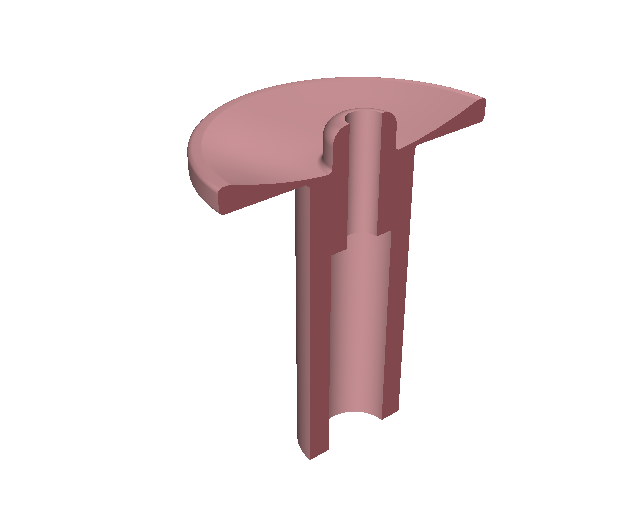
\includegraphics[width=0.55\linewidth]{section.png}
  \begin{minipage}{0.9\linewidth}
    \figcap{P1 shown in section, revealing the internal flow path: the constant-diameter lumen, the step out to the socket bore that grips the handpiece, the internal seating shoulder, and the shallow concave dish with its central nose. The darker faces are the cut plane. The shallowness of the dish relative to the flange width is the conformity concern described above.}
  \end{minipage}
\end{figure}

\section{Acceptance criteria worth adding}

The bench checks in Section 9 are all qualitative, which means none of them can objectively pass or fail. The following additions would make the prototype set genuinely conclusive.

\vspace{0.4em}
\begin{center}
\small
\begin{tabular}{@{}p{0.27\linewidth}p{0.38\linewidth}p{0.27\linewidth}@{}}
\toprule
\textbf{Measure} & \textbf{Why it matters} & \textbf{First estimate} \\
\midrule
Hold force to maintain the seal & The central usability question, currently unmeasured & About 16\,N (1.7\,kgf) on the 50\,mm flange at a 1\,m head; about 20\,N on the 55\,mm \est \\
\addlinespace
Leakage volume, as mL leaked per mL delivered & Makes ``reduce leakage'' testable & Set a target, for example under 5\,\% \\
\addlinespace
Outlet area relative to lumen area & Turns ``no fine jet'' into a specification & Outlet area $\geq$ lumen area \\
\addlinespace
Delivery time for the intended volume & A nozzle that is too slow is clinically unusable & About 9\,s per 500\,mL \est \\
\addlinespace
Water temperature, in the instructions for use & Cold water causes cramping & Body temperature \\
\addlinespace
Release and peel-off behaviour & Suction is forbidden but no feature currently prevents it & Add a small pull tab on a non-contact surface so it peels from one edge \\
\bottomrule
\end{tabular}
\end{center}
\vspace{0.6em}

\noindent The hold force figure deserves emphasis. Roughly 1.7\,kgf sustained is manageable for a caregiver over a minute or two, but it is real physical work, and it determines whether frail patients or those self-administering can use the device at all. It is also easy to measure early: press a printed rigid part against a kitchen scale to the point of a visually complete seal and read the value.

\section{Clinical context and honest limitations}

\subsection*{What supports the concept}

The strongest argument in the design's favour is that the external-hold principle is already in clinical use. Cone-tip irrigation systems are held externally against the anus, and the published rationale is that the external hold avoids provoking the reflex rectal contractions that balloon inflation can trigger. Every dominant transanal irrigation product otherwise inserts, so a well-engineered non-inserting nozzle addresses a real gap.

The patient groups are well defined and substantial: neurogenic bowel dysfunction arising from spinal cord injury, spina bifida, multiple sclerosis and cerebral palsy; low anterior resection syndrome and other post-rectal-surgery states; and patients with fissures, haemorrhoids, strictures or recent anorectal surgery for whom insertion is painful or contraindicated. You will judge this population better than any literature I can cite, and if the idea came from patients in your own clinic, that is the most valuable evidence in the project.

\subsection*{What to stay honest about}

\begin{itemize}
  \item \textbf{Leakage is an expected failure mode,} not an edge case. Plan the bench protocol to measure it rather than to avoid discovering it.
  \item \textbf{A 0 to 5\,mm nose can only engage the distal external anal sphincter,} the voluntary muscle, not the internal sphincter that supplies most resting tone. Retention assistance will therefore be modest.
  \item \textbf{A cough or Valsalva will break the seal.} Such a manoeuvre raises rectal pressure well above a 1\,m water head \est. Your specification already says ``brief assisted retention,'' which is the right claim. It is worth resisting any drift toward describing this as a retention device.
  \item \textbf{Demand for a non-inserting device is inferred rather than demonstrated.} The populations above currently use inserting systems. The reasoning that insertion is painful or contraindicated for a subset is sound, but it remains an inference until you test it with patients.
\end{itemize}

\section{Reusable, single use, or biodegradable}

\subsection*{Reprocessing is the reusable design's weak point}

A 6\,mm lumen roughly 55\,mm long, combined with a socket that closes around the steel spout, creates an occluded space that cannot be reliably brush-cleaned or visually inspected between patients. Silicone autoclaves well, but sterilisation does not substitute for cleaning, and residual bioburden in narrow lumens is the classic reprocessing failure. Repeated autoclave cycles will also gradually relax the push-fit interference, which eventually presents as a leak at the silicone-to-steel joint.

A useful distinction here is between \textbf{single use} and \textbf{single-patient use}. Shared use between patients in a hospital argues strongly for a disposable. A patient reusing their own device at home is a materially easier risk case. You may ultimately want both: a disposable version for the ward and a durable single-patient version for home use.

\subsection*{If single use, the material changes}

Commercially available disposable enema and rectal tips are moulded PVC, ethylene-oxide sterilised and explicitly labelled for single use. A granted patent in this device area names polyurethane as the preferred material, with silicone and SEBS listed only as alternatives. For a disposable, the realistic route is a moulded thermoplastic elastomer or medical PVC at a comfortable durometer, not silicone.

\subsection*{Biodegradable options: not yet viable}

I looked specifically for a polymer that is soft, safe for short skin and mucosal contact, and mouldable. Nothing currently meets all three.

\vspace{0.4em}
\begin{center}
\small
\begin{tabular}{@{}p{0.22\linewidth}p{0.70\linewidth}@{}}
\toprule
\textbf{Candidate} & \textbf{Assessment} \\
\midrule
PLA and PLA blends & Rigid engineering plastics. Even a toughened PLA/PHBV/PCL blend shows a Young's modulus near 950\,MPa, which is roughly three to four orders of magnitude stiffer than Shore A 10 to 20 silicone. Improved ductility is not the same as softness. \\
\addlinespace
PHA, PHB, PHBV & Characterised on the Shore D scale, semicrystalline and stiff. Moulded, unoriented parts would be brittle rather than soft. \\
\addlinespace
Polycaprolactone & Softer than PLA, but degrades over two to four years, which defeats the purpose. \\
\addlinespace
Soft biodegradable elastomers & The one genuinely soft candidate found, a photo-crosslinked PLA-PEG-PLA system, is a UV-cured thermoset that cannot be injection moulded, and has only in-vitro cytocompatibility data with no ISO 10993 mucosal testing. \\
\addlinespace
Water-dispersible or flushable & Self-defeating in a water-delivery device, and flushing soft polymer parts is undesirable for sewer systems. \\
\bottomrule
\end{tabular}
\end{center}
\vspace{0.6em}

\noindent This verdict rests on the absence of qualifying safety data rather than on evidence of harm. If the environmental goal matters to you, two honest interim positions are available: a recyclable single-material thermoplastic elastomer disposable, or a durable single-patient silicone device supported by a take-back scheme. Both are defensible without putting an untested polymer against mucosa.

\section{Making the first prototype}

I looked hard for a Bangalore supplier who could mould a soft platinum-cured silicone part in quantities of two to four, and I was unable to confirm one against primary sources. That is a genuine limitation of searching from outside the city rather than proof that none exists. This trade often operates by phone and personal visit with little web presence, so a morning spent in Peenya or Bommasandra may well succeed where searching did not.

What Bangalore does clearly offer is the first half of the job: printing an accurate rigid master.

\vspace{0.4em}
\begin{center}
\small
\begin{tabular}{@{}p{0.21\linewidth}p{0.20\linewidth}p{0.49\linewidth}@{}}
\toprule
\textbf{Option} & \textbf{Location} & \textbf{What it offers} \\
\midrule
Criador Labs & HRBR Layout, Bangalore & ISO 13485 certified medical-device product-innovation studio, SLA and SLS printing. The strongest local partner for in-person work, though silicone casting is not among its stated capabilities. \\
\addlinespace
iamRapid & HSR Layout, Bangalore & Working SLA resin printing service for fast, inexpensive masters. No silicone capability. \\
\addlinespace
IISc CPDMED & IISc campus & MedTech incubator with rolling admissions whose stated eligibility includes industry professionals. The most credible institutional route locally. \\
\addlinespace
Spectroplast & Zurich, ships internationally & Prints finished parts in true silicone with no tooling. Its TrueSil A20 grade is exactly Shore 20A, orders start at one unit, and it is the only supplier whose ISO 10993 data I could verify. \\
\bottomrule
\end{tabular}
\end{center}
\vspace{0.6em}

\noindent For completeness: C-CAMP's rapid prototyping facility is a microfluidics unit for diagnostic chips rather than a soft-part moulder, and Protolabs offers medical silicone only at Shore A52, which is far too firm for this application.

\textbf{Suggested approach.} Print rigid masters locally this week from the attached files and check them by hand. Rigid parts cannot test sealing, but they will immediately tell you whether the socket fits your steel handpiece, how the flange diameter feels, and how the flange sits against the cleft. That is a few thousand rupees and a few days, in person, and it is worth doing before ordering anything in silicone. Once the geometry settles, order soft parts from Spectroplast, or cast locally into a printed mould using a platinum-cure stock such as Smooth-On Dragon Skin 15 or 20, which matches the target hardness.

\section{The CAD files}

Because the part is a solid of revolution and your specification already fixes every dimension, the model is generated from a short parametric script rather than drawn by hand. Every dimension is a named variable, so producing a new variant means changing one number and re-running it.

\vspace{0.4em}
\begin{center}
\small
\begin{tabular}{@{}llll@{}}
\toprule
\textbf{File} & \textbf{Flange} & \textbf{Nose projection} & \textbf{Purpose} \\
\midrule
\texttt{nozzle\_P1.step} & 50\,mm & 3.00\,mm & Baseline \\
\texttt{nozzle\_P2.step} & 55\,mm & 3.00\,mm & Enhanced external seal \\
\texttt{nozzle\_P3.step} & 50\,mm & 0.00\,mm & Flush, fully non-inserting \\
\texttt{nozzle\_P4.step} & 50\,mm & 5.00\,mm & Maximum allowable projection \\
\bottomrule
\end{tabular}
\end{center}
\vspace{0.6em}

\begin{figure}[H]
  \centering
  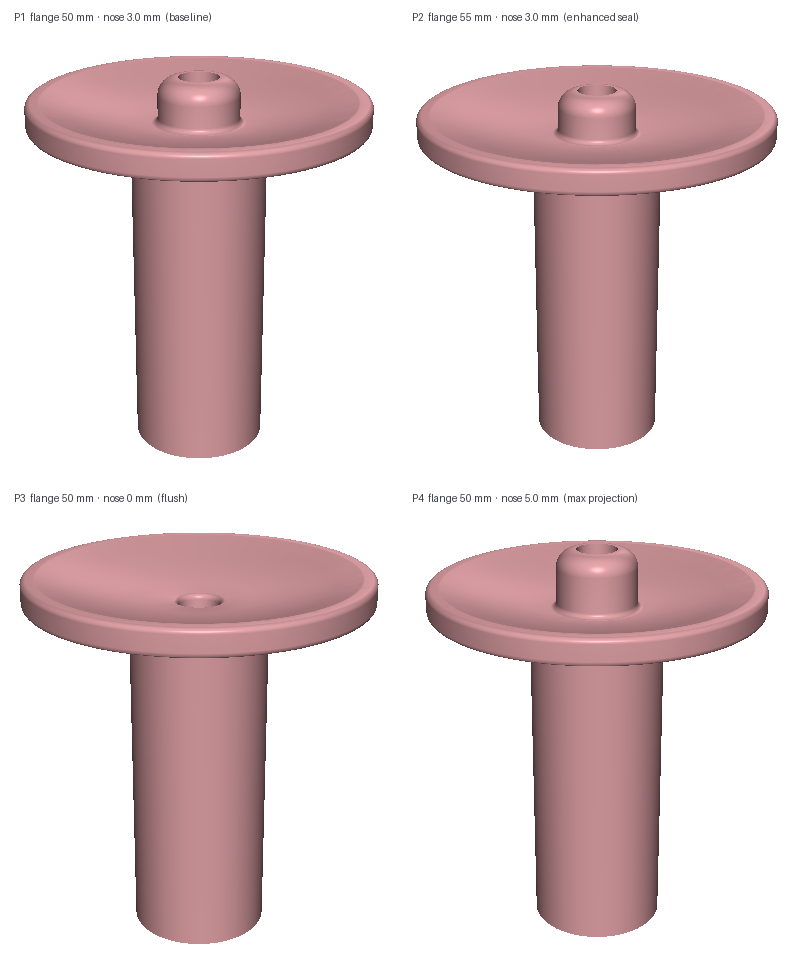
\includegraphics[width=0.78\linewidth]{views_grid.png}
  \begin{minipage}{0.9\linewidth}
    \figcap{The four prototype variants, generated from the accompanying CAD files. P2 carries the wider 55\,mm flange; P3 is the flush, fully non-inserting version; P4 has the maximum 5\,mm nose projection.}
  \end{minipage}
\end{figure}

\noindent Each file was checked rather than assumed: flange diameter and nose projection are verified against the intended values, the internal flow path is confirmed open from end to end, and the models were rendered and compared against Figure 1 in your specification.

Two points for whoever quotes the work. First, \textbf{the socket bore is currently a placeholder}. It cannot be finalised until the steel handpiece spout is measured, which remains the one genuine blocker in the project. Second, these are design-intent models: a production mould additionally needs draft angles, parting-line placement and shrinkage compensation, which the moulder will add in their own CAD. That is normal, and it is what Section 7 of your specification already asks them to supply.

\section{Suggested sequence}

\begin{enumerate}
  \item Change the outlet to a diffusing geometry, and make Shore A 10 the baseline hardness. Both are free now.
  \item Add the quantitative acceptance criteria from Section 4, particularly hold force and leakage volume.
  \item \textbf{Measure the steel handpiece spout} and set the socket bore. Nothing can be finalised without this.
  \item Print rigid masters locally and check fit and cleft geometry by hand.
  \item Order soft silicone parts only once the geometry has settled.
  \item Defer the disposable material and biodegradability decisions until the shape is proven. Choosing a manufacturing material before validating the geometry optimises the wrong end of the problem.
\end{enumerate}

\vspace{0.5em}
\noindent Bench and anatomical-model testing only, as your specification already states. Nothing in this review changes that.

\section*{\sffamily\color{accent} Appendix A: One intellectual property note}

There is a granted United States patent, US 9,227,006 B2, titled ``Non-penetrating nozzle,'' which describes an enema nozzle that seals externally against tissue surrounding the orifice without penetrating it. Its independent claim covers a nozzle with a projecting rim and a continuous side wall that the surrounding tissue conforms to in order to form a seal, and a further claim covers the method of pressing such a nozzle against the orifice without penetrating it.

Two points make this manageable. First, \textbf{there is no Indian member of this patent family}: the international application has ceased, the European application was withdrawn, and only the United States grant remains active, with an expiry in 2032. Manufacture and sale in India therefore appear unaffected. Second, there is no evidence the patent holder ever commercialised a product.

I am not qualified to give legal advice, and this is worth thirty minutes with a patent attorney before any United States ambitions. It is also useful in the other direction: because the general concept is already published, any patent application of your own would need to rest on the specific improvements, such as the sealing geometry, the cleft-conforming skirt or the diffusing outlet, rather than on the non-inserting principle itself.

\section*{\sffamily\color{accent} Appendix B: What a manufacturer will need}

Your Section 11 list is already good. In practice the following is what unblocks a quotation:

\begin{itemize}
  \item The STEP files accompanying this document.
  \item The actual steel handpiece, or a dimensioned drawing of its outlet spout including outside diameter, wall thickness and any taper. This is the item that currently blocks everything.
  \item The material specification: platinum-cured silicone, target Shore A 10 to 20, with a request for the grade's technical data sheet and ISO 10993 documentation.
  \item Quantity stated as two to four prototype variants, explicitly not a production mould.
  \item A request for a tolerance proposal on the outlet, lumen, flange and connector.
  \item Confirmation that patient-contact surfaces will be free of flash, seams, support marks and parting-line witness, and that the lumen will be unobstructed.
  \item A non-disclosure agreement before the drawings circulate.
\end{itemize}

\vspace{1.2em}
\noindent\textcolor{rule}{\rule{\linewidth}{0.8pt}}
\vspace{0.5em}

\noindent{\footnotesize\color{slate} \textbf{On sources and limits.} Factual claims in this review were checked against primary sources, including the published regulation and patent texts, peer-reviewed materials and clinical literature, and manufacturers' own documentation. Figures marked \est\ are my own first-order calculations from the dimensions in your specification, intended to size the problem rather than to serve as engineering results, and should be verified before they inform a design decision. This document is an engineering and materials review. It is not clinical, legal or regulatory advice, and on the clinical questions your judgement supersedes anything written here.}

\end{document}
